\documentclass[11pt,a4paper]{article}
\usepackage[utf8]{inputenc}
\usepackage[T1]{fontenc}
\usepackage[margin=0.85in]{geometry}
\usepackage{amsmath,amssymb,amsfonts,amsthm}
\usepackage{booktabs,multirow,tabularx}
\usepackage{xcolor}
\usepackage{hyperref}
\usepackage{microtype}
\usepackage{fancyhdr}
\usepackage{tcolorbox}
\usepackage{titlesec}
\usepackage{enumitem}
\usepackage{tikz}
\usetikzlibrary{shapes.geometric, arrows, positioning, calc}

% Color Definitions
\definecolor{CDCBlue}{HTML}{003366}
\definecolor{SlateBlue}{HTML}{2B6CB0}
\definecolor{DarkRed}{HTML}{9B2C2C}
\definecolor{LightGrey}{HTML}{F8FAFC}
\definecolor{BorderGrey}{HTML}{CBD5E0}
\definecolor{CodeBg}{HTML}{EDF2F7}

% Hyperref Setup
\hypersetup{
    colorlinks=true,
    linkcolor=CDCBlue,
    citecolor=SlateBlue,
    urlcolor=SlateBlue,
    pdftitle={CDC Cyclospora cayetanensis Legacy Pipeline Audit: WHAT, WHY, HOW},
    pdfauthor={CDC Workflow Modernization Initiative}
}

% Page Header & Footer
\pagestyle{fancy}
\fancyhf{}
\rhead{\textcolor{SlateBlue}{\small \textbf{\textit{Cyclospora cayetanensis} Legacy Pipeline Audit}}}
\lhead{\textcolor{CDCBlue}{\small \textbf{CDC Technical Documentation}}}
\cfoot{\thepage}
\renewcommand{\headrulewidth}{0.4pt}
\setlength{\headheight}{14pt}

% Section & Title Formatting
\titleformat{\section}{\large\bfseries\color{CDCBlue}}{\thesection.}{0.5em}{}[\titlerule]
\titleformat{\subsection}{\bfseries\color{SlateBlue}}{\thesubsection.}{0.5em}{}
\titleformat{\subsubsection}{\bfseries\color{CDCBlue}}{\thesubsubsection.}{0.5em}{}

% Custom Paragraph Formatting
\titleformat{\paragraph}[hang]{\bfseries\color{CDCBlue}}{}{0pt}{}[\vspace{0.2em}]
\titlespacing*{\paragraph}{0pt}{0.6em}{0.4em}

% Custom TColorBox Setup
\tcbuselibrary{skins,breakable}
\newtcolorbox{conceptbox}[1]{
    colback=LightGrey,
    colframe=CDCBlue,
    fonttitle=\bfseries\color{white},
    coltitle=white,
    title=#1,
    arc=1.5mm,
    boxrule=0.8pt,
    left=8pt,right=8pt,top=6pt,bottom=6pt,
    breakable
}

\newtcolorbox{warningbox}[1]{
    colback=LightGrey,
    colframe=DarkRed,
    fonttitle=\bfseries\color{white},
    coltitle=white,
    title=#1,
    arc=1.5mm,
    boxrule=0.8pt,
    left=8pt,right=8pt,top=6pt,bottom=6pt,
    breakable
}

\title{\vspace{-1.5cm}\Huge \textbf{\color{CDCBlue} Architecture \& Operational Audit of the Original CDC \textit{Cyclospora cayetanensis} Genotyping Pipeline}\\[0.4em]
\Large \textbf{\color{SlateBlue} Comprehensive Technical Breakdown: WHAT, WHY, and HOW}}

\author{\textbf{CDC Workflow Modernization Initiative} \\ BRC-Analytics \& Advanced Agentic Coding Team}
\date{August 11, 2026}

\begin{document}

\maketitle

\begin{abstract}
\noindent \textit{Cyclospora cayetanensis} is an obligate human coccidian parasite responsible for annual seasonal outbreaks of diarrheal disease linked to contaminated fresh produce (e.g., cilantro, basil, berries, and bagged salad mixes). Due to the lack of \textit{in vitro} culture systems and the complex, polyploid/multi-strain nature of clinical infections, molecular surveillance relies on deep targeted multi-locus sequence typing (MLST). This document provides an exhaustive technical audit of the original CDC High Sierra ALPHA release workflow. For each core module and algorithmic component, we state \textbf{WHAT} the algorithm does, explain its operational intent, and then detail all associated \textbf{ISSUES AND LIMITATIONS} with mathematical proofs, failure paradoxes, and concrete epidemiological examples.
\end{abstract}

\section{System Overview: WHAT the Pipeline Does}

The CDC \textit{Cyclospora cayetanensis} genotyping pipeline is an automated computational architecture designed to ingest raw Illumina amplicon sequencing reads from patient clinical stool specimens and output outbreak cluster assignments.

\begin{figure}[h]
\centering
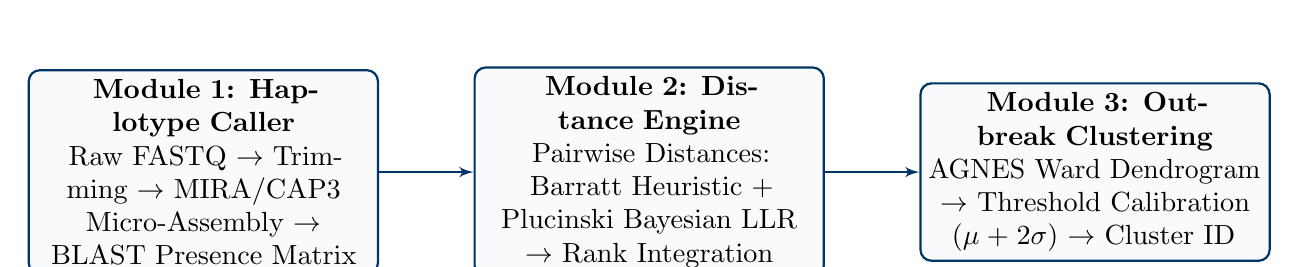
\begin{tikzpicture}[node distance=1.5cm, auto, >=latex', every node/.style={transform shape}]
    \tikzstyle{block} = [rectangle, draw=CDCBlue, fill=LightGrey, thick, text width=4.2cm, align=center, rounded corners, minimum height=1.2cm]
    \tikzstyle{line} = [draw, ->, thick, CDCBlue]
    
    \node [block] (m1) {\textbf{Module 1: Haplotype Caller}\\Raw FASTQ $\rightarrow$ Trimming $\rightarrow$ MIRA/CAP3 Micro-Assembly $\rightarrow$ BLAST Presence Matrix};
    \node [block, right=1.2cm of m1] (m2) {\textbf{Module 2: Distance Engine}\\Pairwise Distances: Barratt Heuristic + Plucinski Bayesian LLR $\rightarrow$ Rank Integration};
    \node [block, right=1.2cm of m2] (m3) {\textbf{Module 3: Outbreak Clustering}\\AGNES Ward Dendrogram $\rightarrow$ Threshold Calibration ($\mu + 2\sigma$) $\rightarrow$ Cluster ID};
    
    \path [line] (m1) -- (m2);
    \path [line] (m2) -- (m3);
\end{tikzpicture}
\caption{High-Level Architectural Workflow of the Legacy CDC Pipeline across Modules 1, 2, and 3.}
\label{fig:arch}
\end{figure}

As shown in Figure~\ref{fig:arch}, the pipeline operates across three primary stages:
\begin{enumerate}[leftmargin=*]
    \item \textbf{Module 1 (Haplotype Caller \& Micro-Assembler):} Converts raw paired-end Illumina FASTQ reads into clean amplicon haplotype profiles across 8 targeted genomic loci.
    \item \textbf{Module 2 (Multi-Locus Distance Matrix Engine):} Evaluates pairwise genetic divergence among specimens using a dual-ensemble metric combining Barratt's Heuristic Distance and Plucinski's Bayesian Log-Likelihood Ratio.
    \item \textbf{Module 3 (Outbreak Cluster Finder):} Performs agglomerative hierarchical clustering (Ward's AGNES method) and calibrates distance thresholds to isolate discrete epidemiological outbreak clusters.
\end{enumerate}

\section{Public Health Imperative: WHY the Pipeline Exists}

\begin{conceptbox}{Epidemiological Purpose \& Operational Goals}
\begin{itemize}[leftmargin=*]
    \item \textbf{Outbreak Cluster Resolution:} Distinguishes sporadic background cyclosporiasis cases from widespread, multi-state foodborne outbreaks.
    \item \textbf{Traceback Support:} Provides molecular evidence matching patient isolates from different geographic regions to specific agricultural sources (e.g., imported fresh basil, cilantro, or raspberries).
    \item \textbf{Overcoming Non-Culturability:} Because \textit{C. cayetanensis} cannot be cultured in cell lines or laboratory animals, public health surveillance relies entirely on direct molecular typing of oocyst DNA extracted from stool or food washes.
\end{itemize}
\end{conceptbox}

\section{Methodological Audit: HOW Each Module Operates}

\subsection{Haplotype Calling \& Read Processing (Module 1)}

\subsubsection{Operational Mechanics (WHAT the Algorithm Does)}
In Module 1, an \textbf{allele} is defined as a unique, discrete consensus DNA sequence string (a full amplicon sequence variant or ``haplotype'') called across one of 8 targeted MLST genomic loci (\texttt{Mt\_Cmt}, \texttt{Mt\_MSR}, \texttt{Nu\_360i2}, \texttt{Nu\_378}, \texttt{Nu\_CDS1--4}).
Raw FASTQ reads are trimmed using \texttt{cutadapt}, assembled at \texttt{Mt\_Cmt} using MIRA 4.0.2 / CAP3, clustered into centroid sequences at 99\% sequence identity using \texttt{CD-HIT-est}, and matched against a reference database using \texttt{blastn} with \texttt{-qcov\_hsp\_perc 100}. Module 1 outputs a binary presence/absence matrix where an allele is declared \textbf{PRESENT} (\texttt{X}) if it receives $\ge 10$ supporting reads.

\begin{figure}[h]
\centering
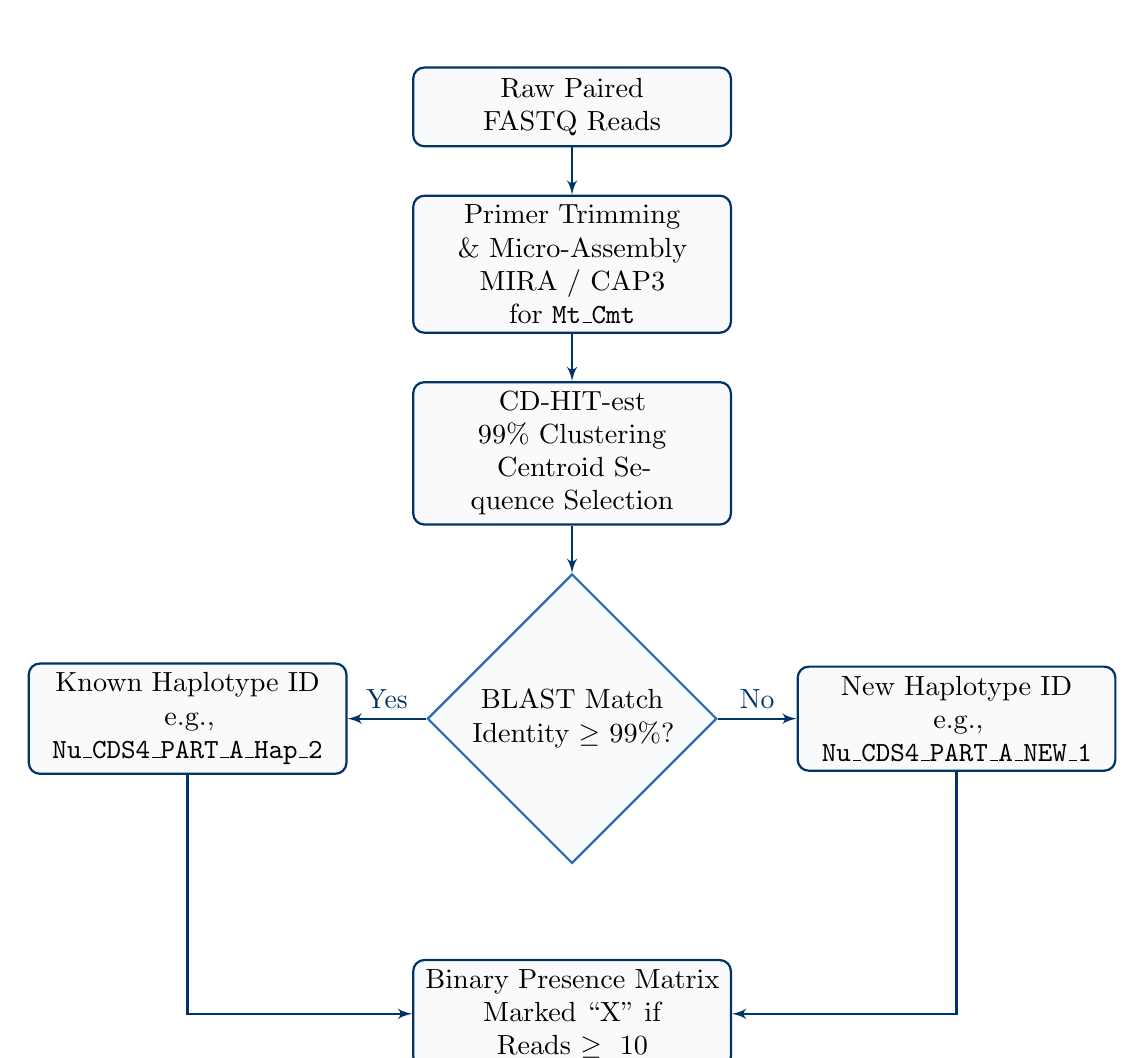
\begin{tikzpicture}[node distance=1.6cm, auto, >=latex', every node/.style={transform shape}]
    \tikzstyle{block} = [rectangle, draw=CDCBlue, fill=LightGrey, thick, text width=3.8cm, align=center, rounded corners, minimum height=1.0cm]
    \tikzstyle{decision} = [diamond, draw=SlateBlue, fill=LightGrey, thick, text width=2.8cm, align=center, inner sep=1pt]
    \tikzstyle{line} = [draw, ->, thick, CDCBlue]
    
    \node [block] (reads) {Raw Paired FASTQ Reads};
    \node [block, below=0.6cm of reads] (trim) {Primer Trimming \& Micro-Assembly\\MIRA / CAP3 for \texttt{Mt\_Cmt}};
    \node [block, below=0.6cm of trim] (cdhit) {CD-HIT-est 99\% Clustering\\Centroid Sequence Selection};
    \node [decision, below=0.6cm of cdhit] (blast) {BLAST Match\\Identity $\ge 99\%$?};
    \node [block, left=1.0cm of blast] (known) {Known Haplotype ID\\e.g., \texttt{Nu\_CDS4\_PART\_A\_Hap\_2}};
    \node [block, right=1.0cm of blast] (new) {New Haplotype ID\\e.g., \texttt{Nu\_CDS4\_PART\_A\_NEW\_1}};
    \node [block, below=1.2cm of blast] (matrix) {Binary Presence Matrix\\Marked ``X'' if Reads $\ge 10$};
    
    \path [line] (reads) -- (trim);
    \path [line] (trim) -- (cdhit);
    \path [line] (cdhit) -- (blast);
    \path [line] (blast) -- node [above] {Yes} (known);
    \path [line] (blast) -- node [above] {No} (new);
    \path [line] (known) |- (matrix);
    \path [line] (new) |- (matrix);
\end{tikzpicture}
\caption{Operational Workflow for Allele / Haplotype Calling and BLAST Classification in Module 1.}
\label{fig:allele_calling}
\end{figure}

\begin{table}[h]
\centering
\small
\caption{The 8 Targeted MLST Loci and Haplotype Naming Conventions}
\label{tab:loci}
\begin{tabularx}{\textwidth}{l p{2.8cm} p{3.2cm} p{4.2cm} c}
\toprule
\textbf{Locus} & \textbf{Compartment} & \textbf{Biological Feature} & \textbf{Example Allele Label} & \textbf{Target Length} \\
\midrule
\texttt{Mt\_Cmt} & Mitochondrial & Intergenic junction repeat & \texttt{\small Mt\_Cmt\_Junction\_Hap\_3} & 200--600 bp \\
\texttt{Mt\_MSR} & Mitochondrial & Sequence repeat locus & \texttt{\small Mt\_MSR\_PART\_A\_Hap\_1} & $\approx 250$ bp \\
\texttt{Nu\_360i2} & Nuclear Chrom. & Intron 2 sequence window & \texttt{\small Nu\_360i2\_PART\_A\_Hap\_2} & $\approx 360$ bp \\
\texttt{Nu\_378} & Nuclear Chrom. & Hyper-variable locus 378 & \texttt{\small Nu\_378\_PART\_A\_Hap\_4} & $\approx 300$ bp \\
\texttt{Nu\_CDS1} & Nuclear Chrom. & Coding sequence window 1 & \texttt{\small Nu\_CDS1\_PART\_A\_Hap\_1} & $\approx 400$ bp \\
\texttt{Nu\_CDS2} & Nuclear Chrom. & Coding sequence window 2 & \texttt{\small Nu\_CDS2\_PART\_A\_Hap\_1} & $\approx 450$ bp \\
\texttt{Nu\_CDS3} & Nuclear Chrom. & Coding sequence window 3 & \texttt{\small Nu\_CDS3\_PART\_A\_Hap\_1} & $\approx 350$ bp \\
\texttt{Nu\_CDS4} & Nuclear Chrom. & Coding sequence window 4 & \texttt{\small Nu\_CDS4\_PART\_A\_Hap\_1} & $\approx 400$ bp \\
\bottomrule
\end{tabularx}
\end{table}

\subsubsection{Issues \& Limitations (Short-Read Query vs. Subject Coverage Flaw)}
\begin{warningbox}{Short-Read Query vs. Subject Coverage Vulnerability}
Module 1 executes \texttt{blastn} using \texttt{-qcov\_hsp\_perc 100}. In BLAST syntax, \texttt{-qcov\_hsp\_perc 100} checks 100\% of the \textbf{Query Read} length, NOT 100\% of the \textbf{Subject Reference Amplicon}! \\
If a truncated 40-bp read fragment survives trimming without a minimum length filter (\texttt{cutadapt -m 200}), and aligns to a conserved 40-bp motif within a 400-bp reference sequence, its Query Coverage is 100\% ($40/40\text{ bp} = 100\%$). BLAST passes this hit as 100\% identical, even though Subject Coverage is only 10\% ($40/400\text{ bp}$). If 10 such short non-specific fragments align, Module 1 erroneously declares the entire 400-bp haplotype \textbf{PRESENT} (\texttt{X}), generating spurious allele calls!
\end{warningbox}

\subsection{Barratt's Heuristic Distance Engine (Module 2)}

To handle Multiplicity of Infection (MOI > 1) where patients carry multiple alleles ($v_1, v_2$) without requiring full clonal phasing, Joel Barratt designed a custom heuristic scoring function.
Let $n_{\text{min}} = \min(|v_1|, |v_2|)$, total union size $x = |v_1 \cup v_2|$, and shared allele count $y = |v_1 \cap v_2|$.

\begin{figure}[h]
\centering
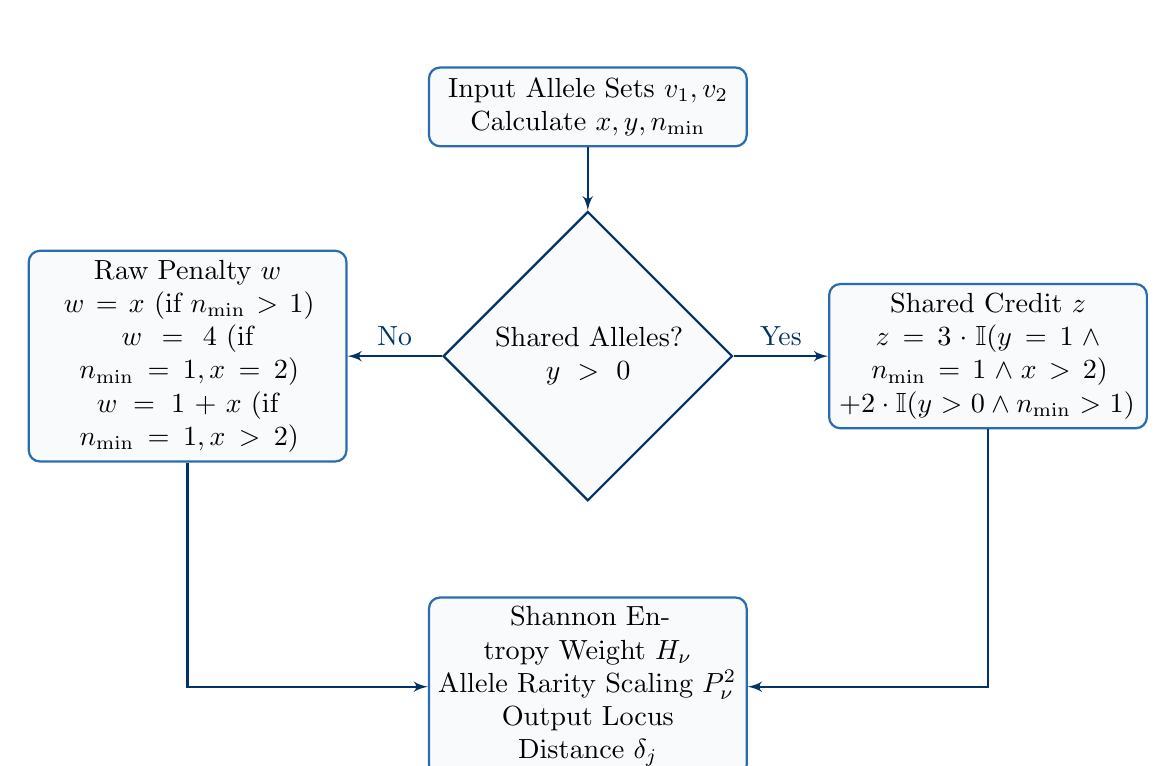
\begin{tikzpicture}[node distance=1.8cm, auto, >=latex', every node/.style={transform shape}]
    \tikzstyle{decision} = [diamond, draw=CDCBlue, fill=LightGrey, thick, text width=2.8cm, align=center, inner sep=1pt]
    \tikzstyle{block} = [rectangle, draw=SlateBlue, fill=LightGrey, thick, text width=3.8cm, align=center, rounded corners, minimum height=1.0cm]
    \tikzstyle{line} = [draw, ->, thick, CDCBlue]
    
    \node [block] (in) {Input Allele Sets $v_1, v_2$\\Calculate $x, y, n_{\text{min}}$};
    \node [decision, below=0.8cm of in] (shared) {Shared Alleles?\\$y > 0$};
    \node [block, left=1.2cm of shared] (unshared_w) {Raw Penalty $w$\\$w = x$ (if $n_{\text{min}} > 1$)\\$w = 4$ (if $n_{\text{min}}=1, x=2$)\\$w = 1+x$ (if $n_{\text{min}}=1, x>2$)};
    \node [block, right=1.2cm of shared] (shared_z) {Shared Credit $z$\\$z = 3\cdot\mathbb{I}(y=1 \land n_{\text{min}}=1 \land x>2)$\\$+ 2\cdot\mathbb{I}(y>0 \land n_{\text{min}}>1)$};
    \node [block, below=1.2cm of shared] (final_dist) {Shannon Entropy Weight $H_\nu$\\Allele Rarity Scaling $P_\nu^2$\\Output Locus Distance $\delta_j$};
    
    \path [line] (in) -- (shared);
    \path [line] (shared) -- node [above] {No} (unshared_w);
    \path [line] (shared) -- node [above] {Yes} (shared_z);
    \path [line] (unshared_w) |- (final_dist);
    \path [line] (shared_z) |- (final_dist);
\end{tikzpicture}
\caption{Decision Tree Logic of Barratt's Heuristic Distance Calculation per Locus.}
\label{fig:barratt_flow}
\end{figure}

\subsubsection{Raw Locus Divergence Penalty (\texorpdfstring{$w$}{w})}
\paragraph{Operational Mechanics (WHAT the Algorithm Does):}
The algorithm penalizes total allele diversity $x$. The penalty $w$ depends on whether $n_{\text{min}} = 1$ (single-allele specimen) or $n_{\text{min}} > 1$ (multi-allele specimen):
\begin{equation}
w = \begin{cases} 
x & \text{if } n_{\text{min}} > 1 \\
4 & \text{if } n_{\text{min}} = 1 \text{ and } x = 2 \\
1 + x & \text{if } n_{\text{min}} = 1 \text{ and } x > 2 
\end{cases}
\end{equation}

\paragraph{Issues \& Limitations (Unbounded Penalty Scaling Flaw):}
\begin{warningbox}{Unbounded Raw Penalty Scaling Flaw ($\delta_{\text{raw}} > 4.0$)}
While $w = 4.0$ serves as a reference ceiling for simple single-allele vs. diploid pairs ($n_{\text{min}}=1, x=2$), when comparing complex multi-strain co-infections ($n_{\text{min}} > 1$ or $x > 3$) with zero shared alleles ($y = 0$), \textbf{the raw distance $\delta_{\text{raw}} = w$ is completely uncapped and scales unboundedly with total union size $x$!}\\
For example, if two patients each have 3 un-shared alleles ($x = 6, y = 0$), $\delta_{\text{raw}} = w = x = \mathbf{6.0}$. If one patient has 5 un-shared alleles ($x = 6, n_{\text{min}} = 1, y = 0$), $\delta_{\text{raw}} = 1 + x = \mathbf{7.0}$. This unbounded scaling causes high-MOI loci to produce runaway distances that completely overwhelm and distort the multi-locus sum across all 8 loci!
\end{warningbox}

\subsubsection{Shared Allele Reduction (\texorpdfstring{$z$}{z}) \& Net Raw Distance (\texorpdfstring{$\delta_{\text{raw}}$}{delta\_raw})}
\paragraph{Operational Mechanics (WHAT the Algorithm Does):}
If specimens share at least one allele ($y > 0$), a reduction term $z$ offsets the divergence penalty:
\begin{equation}
z = 3 \cdot \mathbb{I}(y = 1 \land n_{\text{min}} = 1 \land x > 2) + 2 \cdot \mathbb{I}(y > 0 \land n_{\text{min}} > 1)
\end{equation}
\begin{equation}
\delta_{\text{raw}} = \begin{cases}
w & \text{if } y = 0 \text{ (zero shared alleles)} \\
4 - z & \text{if } y > 0 \text{ (some shared alleles)}
\end{cases}
\end{equation}

\paragraph{Issues \& Limitations (The High MOI Paradox):}
If Patient A has a single strain ($v_A = \{X\}$) and Patient B has a mixed infection of Outbreak Strain $X$ + background strains $Y, Z$ ($v_B = \{X, Y, Z\}$), $x = |v_A \cup v_B| = 3$. The heuristic assigns a large penalty $\delta_{\text{raw}} = 1 + x = 4$, \textbf{falsely excluding Patient B from the outbreak cluster} purely because they ingested secondary background strains!

\subsubsection{Shannon Entropy Information Weighting (\texorpdfstring{$H_\nu$}{H\_nu})}

\paragraph{Operational Mechanics (WHAT the Algorithm Does):}
In Module 2, the raw distance $\delta_{\text{raw}}$ at locus $\nu$ is multiplied by the \textbf{Shannon Entropy ($H_\nu$)} of population allele frequencies $p_k$:
\begin{equation}
H_\nu = -\sum_{k=1}^K p_k \log_2(p_k)
\end{equation}
\begin{equation}
\delta_j = H_\nu \cdot \left[ \delta_{\text{raw}} \cdot \mathbb{I}(\delta_{\text{raw}} > 0) + P_\nu \cdot \mathbb{I}(\delta_{\text{raw}} == 0) \right] \cdot P_\nu
\end{equation}
The CDC's operational intent was to award higher weight to highly polymorphic loci and lower weight to invariant loci.

\paragraph{Issues \& Limitations (Ad-Hoc Weighting \& Inverse Outbreak Paradoxes):}
Multiplying pairwise distance by $H_\nu$ is \textbf{mathematically ad-hoc, statistically unjustified, and fundamentally flawed}:
\begin{enumerate}[leftmargin=*]
    \item \textbf{Information Theory Misapplication:} Shannon Entropy $H_\nu$ measures information disorder/uncertainty (bits) in a signal transmission channel. It is NOT a metric of genetic distance, kinship, or evolutionary divergence. There is zero population genetics theory (e.g., Wright's $F_{ST}$ or coalescent theory) justifying a linear multiplication of pairwise genetic distance by Shannon bits.
    \item \textbf{The Low-Frequency Outbreak Suppression Paradox:} Suppose a critical outbreak marker locus has a single dominant allele ($p_1 = 0.96$) and two rare outbreak variants ($p_2 = 0.02, p_3 = 0.02$).
    \begin{equation}
    H_{\text{outbreak}} = -(0.96 \log_2 0.96 + 2 \cdot 0.02 \log_2 0.02) = \mathbf{0.287 \text{ bits}}
    \end{equation}
    Sharing one of these rare 2\% outbreak variants is \textbf{extremely informative} for epidemiological traceback. However, $H_\nu = 0.287$ \textbf{heavily suppresses} this locus distance by a factor of 3.5$\times$!
    \item \textbf{The High-Noise Background Explosion Paradox:} Conversely, suppose a noisy intron locus has 8 equally frequent background alleles ($p_k = 0.125$).
    \begin{equation}
    H_{\text{noise}} = -8 \cdot (0.125 \log_2 0.125) = \mathbf{3.000 \text{ bits}}
    \end{equation}
    This background noise locus is multiplied by \textbf{3.000 (over 10$\times$ higher weight than the true outbreak marker locus)}, causing random background variation to completely drown out true outbreak signals!
    \item \textbf{Batch-Dependent Metric Space Violation:} Because $H_\nu$ depends on the allele frequency $p_k$ of the active batch, adding 50 unrelated samples to a run alters $H_\nu$ for every locus. As a result, the distance between Specimen A and Specimen B \textbf{changes purely because unrelated samples were added to the batch}, violating the fundamental axiom of pairwise metric spaces ($\text{Dist}(A, B)$ must be invariant to Specimen C).
\end{enumerate}

\subsubsection{Allele Rarity Scaling Factor (\texorpdfstring{$P_\nu$}{P\_nu})}

\paragraph{Operational Mechanics (WHAT the Algorithm Does):}
When specimens share an allele $k$ at locus $\nu$, Barratt scales the shared allele distance by the squared cohort frequency $P_\nu$:
\begin{equation}
P_\nu = \left( \frac{\text{Number of specimens in active batch sharing allele } k}{\text{Total valid specimens in active batch } N} \right)^2
\end{equation}
The intent was to grant greater similarity credit (lower distance) to shared rare alleles.

\paragraph{Issues \& Limitations (The Outbreak Dilution Paradox):}
The quadratic frequency fraction $P_\nu^2 = (\text{count}/N)^4$ introduces \textbf{severe algorithmic failure modes}:
\begin{enumerate}[leftmargin=*]
    \item \textbf{The Outbreak Dilution Paradox (Success Punished by Higher Distances):} Suppose a local health department identifies an early outbreak with 2 patient samples sharing a rare allele \texttt{Hap\_X} ($N=100$).
    \begin{equation}
    P_{\text{early}} = \frac{2}{100} = 0.02 \implies P_{\text{early}}^2 = \mathbf{0.0004} \quad (\text{Tightly Clustered, } \delta_j = 0.0004)
    \end{equation}
    Over the next two weeks, as the outbreak expands and state labs submit 50 more matching patient samples with \texttt{Hap\_X} ($N=150$):
    \begin{equation}
    P_{\text{expanded}} = \frac{52}{150} = 0.347 \implies P_{\text{expanded}}^2 = \mathbf{0.1202} \quad (\mathbf{300\times \text{ Higher Pairwise Distance!}})
    \end{equation}
    \textbf{The Paradox:} As more matching outbreak cases are sequenced, the allele is no longer ``rare'' in the batch. The heuristic \textbf{increases the distance between identical outbreak patients by 300$\times$}, eventually causing late-stage outbreak cases to be \textbf{ejected from the outbreak cluster}!
    \item \textbf{Non-Deterministic Pairwise Distances Across Runs:} Re-running Specimen A and Specimen B in a small state lab batch ($N=20$) vs. a CDC national surveillance batch ($N=500$) alters $P_\nu^2$ by up to 625$\times$. Pairwise distances are not fixed, violating reproducibility requirements.
\end{enumerate}

\subsection{Plucinski's Bayesian Log-Likelihood Ratio Model \& Rank Integration}

\subsubsection{Operational Mechanics: Biological Hypotheses, Input Data Flow \& Distance Generation (WHAT It Does)}

A critical insight into Plucinski's Bayesian model is that \textbf{sequence alignment distances (e.g. SNP counts or percent identity) DO NOT feed INTO the Bayesian calculation}. 

Instead, the Bayesian procedure ingests categorical allele presence vectors ($v_1, v_2$) and cohort allele frequencies ($p_k$), evaluates 3 competing epidemiological hypotheses ($H_0, H_1, H_2$), and \textbf{CREATES} a Bayesian Distance Matrix ($\mathbf{D}_{\text{bayes}}$) which is then rank-integrated with Barratt's heuristic into the final ensemble distance matrix ($\mathbf{D}_{\text{ensemble}}$):

\paragraph{Per-Locus Generative Hypothesis Definitions ($H_0, H_1, H_2$):}
For a specimen pair $(i_1, i_2)$ at locus $j$ with observed allele vectors $v_1, v_2$ and population allele frequencies $p_1, p_2$:
\begin{enumerate}[leftmargin=*]
    \item \textbf{Hypothesis $H_0$ (0 Shared Strains — Unrelated Infections):} Represents the baseline null hypothesis where Patient 1 and Patient 2 contracted completely independent, unrelated infections by randomly sampling parasite strains from the population pool according to frequency $p$. The joint probability of observing all alleles in $v_1$ AND all alleles in $v_2$ independently is:
    \begin{equation}
    L_0^{(j)} = \left( \prod_{a \in v_1} p_a \right) \times \left( \prod_{b \in v_2} p_b \right) \implies \ell_0^{(j)} = \sum_{a \in v_1} \ln p_a + \sum_{b \in v_2} \ln p_b
    \end{equation}
    \item \textbf{Hypothesis $H_1$ (1 Shared Outbreak Strain + Independent Background Strains):} Assumes both patients were exposed to a shared outbreak source that transmitted \textbf{ONE COMMON OUTBREAK STRAIN} carrying allele $k \in v_1 \cap v_2$ (probability $\propto p_k$). Shared allele $k$ is removed from sample 1's product (\texttt{p1[-i]}), while sample 2 retains all alleles (\texttt{p2}):
    \begin{equation}
    L_1^{(j)} = \max_{k \in v_1 \cap v_2} \left[ \left(\prod_{a \in v_1 \setminus \{k\}} p_a\right) \times \left(\prod_{b \in v_2} p_b\right) \right] = \max_{k \in v_1 \cap v_2} \left[ p_k \times \left(\prod_{a \in v_1 \setminus \{k\}} p_a\right) \times \left(\prod_{b \in v_2 \setminus \{k\}} p_b\right) \right]
    \end{equation}
    \begin{equation}
    \ell_1^{(j)} = \max_{k \in v_1 \cap v_2} \left[ \sum_{a \in v_1 \setminus \{k\}} \ln p_a + \sum_{b \in v_2} \ln p_b \right]
    \end{equation}
    \textit{Log-Likelihood Ratio Derivation ($H_1$ vs. $H_0$):} When a single allele $k$ is shared ($v_1 \cap v_2 = \{k\}$), dividing $L_1^{(j)}$ by $L_0^{(j)} = p_k^2 \cdot \prod_{a \neq k} p_a \cdot \prod_{b \neq k} p_b$ cancels all unshared background terms perfectly:
    \begin{equation}
    \text{LLR}_{10} = \ln \left( \frac{L_1^{(j)}}{L_0^{(j)}} \right) = \ln \left( \frac{p_k \cdot \prod_{a \neq k} p_a \cdot \prod_{b \neq k} p_b}{p_k^2 \cdot \prod_{a \neq k} p_a \cdot \prod_{b \neq k} p_b} \right) = \ln \left( \frac{1}{p_k} \right) = -\ln(p_k)
    \end{equation}
    \textit{Behavior When $|v_1 \cap v_2| \ge 2$ Under $H_1$:} If specimens share multiple alleles (e.g. $v_1 \cap v_2 = \{A, B\}$), \texttt{max} selects the single \textbf{rarest matching allele} ($k = \arg\min(p_A, p_B)$), yielding $\text{LLR}_{10} = -\ln(\min(p_A, p_B))$. The secondary matching allele is treated as an unshared background strain, granting zero additional similarity credit under $H_1$! \\
    If $v_1 \cap v_2 = \emptyset$, $\ell_1^{(j)} = \ln \left( \epsilon \cdot \min(p_1 \cup p_2) \right)$ where $\epsilon = 0.3072$ is the missing allele penalty.
    \item \textbf{Hypothesis $H_2$ (2 Shared Outbreak Strains / Clonal Pair):} Assumes both patients were exposed to a shared outbreak source containing \textbf{TWO COMMON OUTBREAK STRAINS} carrying allele pair $(k_1, k_2) \in \text{Pairs}(v_1 \cap v_2)$ generated by \texttt{combn(v, 2)} (probability $\propto p_{k_1} p_{k_2}$):
    \begin{equation}
    L_2^{(j)} = \max_{(k_1, k_2) \in \text{Pairs}(v_1 \cap v_2)} \left[ \left(\prod_{a \in v_1 \setminus \{k_1, k_2\}} p_a\right) \times \left(\prod_{b \in v_2} p_b\right) \right]
    \end{equation}
    \begin{equation}
    \ell_2^{(j)} = \max_{(k_1, k_2) \in \text{Pairs}(v_1 \cap v_2)} \left[ \sum_{a \in v_1 \setminus \{k_1, k_2\}} \ln p_a + \sum_{b \in v_2} \ln p_b \right]
    \end{equation}
    \textit{Log-Likelihood Ratio Derivation ($H_2$ vs. $H_0$):} Under $H_2$, both shared alleles grant rarity surprises: $\text{LLR}_{20} = -\ln(p_{k_1}) - \ln(p_{k_2})$. \\
    \textit{Behavior When $|v_1 \cap v_2| \ge 3$ Under $H_2$:} If specimens share $\ge 3$ alleles (e.g. $\{A, B, C\}$), \texttt{max} selects the single \textbf{rarest 2-allele pair} ($\{k_1, k_2\} = \arg\min (p_{k_1} p_{k_2})$), granting $\text{LLR}_{20} = -\ln(p_{k_1}) - \ln(p_{k_2})$. The 3rd matching allele is \textbf{treated as unshared background noise and penalized}! For haploid mitochondrial loci ($\text{ploidy}=1$), $\ell_2^{(j)} = \ell_1^{(j)}$.
\end{enumerate}

\paragraph{Multi-Locus Summation, Log-Softmax Posteriors \& Rank Integration:}
\begin{enumerate}[leftmargin=*]
    \item \textbf{Multi-Locus Log-Likelihood Summation:} Assuming linkage equilibrium across loci, joint log-likelihoods are summed over all $L$ valid loci:
    \begin{equation}
    \mathbf{L}_m = \sum_{j=1}^L \ell_m^{(j)} \quad \text{for } m \in \{0, 1, 2\}
    \end{equation}
    \item \textbf{Log-Softmax Posterior Probabilities:} Converts multi-locus log-likelihoods into normalized posteriors ($P_0, P_1, P_2$):
    \begin{equation}
    P_m = \frac{\exp(\mathbf{L}_m - \max(\mathbf{L}))}{\sum_{r=0}^2 \exp(\mathbf{L}_r - \max(\mathbf{L}))}
    \end{equation}
    \item \textbf{Bayesian Distance Score ($\mathbf{D}_{\text{bayes}}$):} Converts posteriors into an expected strain dissimilarity score:
    \begin{equation}
    \mathbf{D}_{\text{bayes}}(i_1, i_2) = 0 \cdot P_2 + 1 \cdot P_1 + 2 \cdot P_0 \in [0.0, 2.0]
    \end{equation}
    \item \textbf{Uniform Fractional Rank Integration ($\mathbf{D}_{\text{ensemble}}$):} Converts $\mathbf{D}_{\text{heur}} \in [0, \infty)$ and $\mathbf{D}_{\text{bayes}} \in [0, 2]$ into fractional ranks ($R \in (0, 1]$) and computes their average:
    \begin{equation}
    \mathbf{D}_{\text{ensemble}}(i_1, i_2) = 0.5 \cdot \frac{\text{Rank}(\mathbf{D}_{\text{heur}}(i_1, i_2))}{K} + 0.5 \cdot \frac{\text{Rank}(\mathbf{D}_{\text{bayes}}(i_1, i_2))}{K}
    \end{equation}
    where $K = \frac{N(N-1)}{2}$. $\mathbf{D}_{\text{ensemble}}$ is passed to \textbf{Module 3 for Ward's Hierarchical Clustering}.
\end{enumerate}

\subsubsection{Issues \& Limitations (Audit of Ad-Hoc, Unsound, \& Population Genetics Assumptions)}
While Plucinski's Bayesian framework represents a formal statistical approach, a rigorous mathematical and population genetics audit reveals \textbf{7 major flaws and un-sustained assumptions}:

\begin{enumerate}[leftmargin=*]
    \item \textbf{Implicit Free Recombination (Panmixia) Assumption (Unsound Population Genetics):} Sampling alleles independently both within co-infections ($p_{A_1} \cdot p_{A_2}$) and across loci ($\mathbf{L}_m = \sum \ell^{(j)}$) \textbf{mathematically assumes complete Linkage Equilibrium ($D=0$, free random sexual recombination)}. In reality, \textit{C. cayetanensis} exhibits a predominantly \textbf{clonal or highly selfing population structure} with strong Linkage Disequilibrium (LD) across amplicons. Summing independent log-likelihoods over linked loci over-counts statistical degrees of freedom ($8\times$ too high), causing multi-locus log-likelihoods to explode ($\mathbf{L}_m \pm 100 \dots 1000$) and forcing log-softmax posteriors to collapse to binary $0.0$ or $1.0$, destroying fine-grained probability resolution.
    \item \textbf{Profile Maximum Operator Instead of Bayesian Marginalization (Unsound):} Rather than integrating (summing) over all candidate shared alleles weighted by their prior, $L_1$ takes a hard maximum ($\max_{k}$). This profile likelihood approximation systematically overestimates $L_1$ and underestimates posterior uncertainty.
    \item \textbf{Hardcoded Missing Allele Magic Constant ($\epsilon = 0.3072$) (Ad-Hoc):} When zero alleles are shared ($v_1 \cap v_2 = \emptyset$), $L_1$ falls back to $\ln(\epsilon \cdot \min(p_1 \cup p_2))$ where $\epsilon = 0.3072$ is an uncalibrated, hardcoded magic constant (read from a text file \texttt{EPSILON}). Under zero shared alleles, the probability of sharing an outbreak strain should be 0.0 or depend on explicit sequencing dropout parameters ($p_{\text{drop}}$).
    \item \textbf{Asymmetric Likelihood Implementation Bug (Unsound Code Artifact):} In the original R implementation (\texttt{euk\_bayesian\_fulldataset\_V3.r}, lines 40--41), the denominator product is computed as \texttt{p1[-i]} $\times$ \texttt{p2}. The shared allele $i$ is removed from Patient 1's product but \textbf{left inside Patient 2's product (\texttt{p2})}. This introduces an asymmetric sampling artifact where swapping isolate order shifts distance values.
    \item \textbf{Capped Hypothesis Space ($H_0, H_1, H_2$) in High MOI:} The model evaluates only 3 hypotheses. When two complex co-infections share 3 or 4 distinct strains ($|v_1 \cap v_2| \ge 3$), the algorithm forces the pair into $H_1$ or $H_2$, treating the 3rd and 4th shared alleles as independent background noise and penalizing their log-likelihoods!
    \item \textbf{Arbitrary Distance Linearity ($\mathbf{D}_{\text{bayes}} = 0 P_2 + 1 P_1 + 2 P_0$) (Ad-Hoc):} Assigning exact integer weights $0.0$ ($H_2$), $1.0$ ($H_1$), and $2.0$ ($H_0$) is mathematically ad-hoc. There is zero evolutionary or coalescent theory proving that sharing 1 strain is exactly halfway between sharing 2 strains and sharing 0 strains.
    \item \textbf{Destructive Fractional Rank Integration ($0.5 R_{\text{heur}} + 0.5 R_{\text{bayes}}$) (Ad-Hoc):} Equal 50/50 weighting is an unvalidated heuristic. Furthermore, converting continuous distances into ordinal ranks destroys metric spacing ($0.001$ distance gap vs. $10.0$ distance gap become identical rank steps $1/K$). This distorts Ward's hierarchical clustering (which requires Euclidean metric spaces) into clustering on ordinal rank topologies.
\end{enumerate}

\subsection{AGNES Ward Hierarchical Clustering (Module 3)}

\subsubsection{Operational Mechanics (WHAT the Algorithm Does)}
Module 3 constructs an AGNES (Agglomerative Nesting) dendrogram using Ward's minimum variance method, which minimizes total within-cluster variance $\Delta \text{ESS}$:
\begin{equation}
\Delta \text{ESS}(A, B) = \frac{n_A n_B}{n_A + n_B} \|\mathbf{m}_A - \mathbf{m}_B\|^2
\end{equation}
where $\mathbf{m}_A, \mathbf{m}_B \in \mathbb{R}^{N-1}$ are the cluster mean centroid vectors in the Multidimensional Scaling (MDS) Euclidean coordinate embedding space of $\mathbf{D}_{\text{ensemble}}$. Equivalently, using the Lance-Williams dissimilarity expansion:
\begin{equation}
\|\mathbf{m}_A - \mathbf{m}_B\|^2 = \frac{1}{n_A n_B} \sum_{i \in A} \sum_{j \in B} d(i, j)^2 - \frac{1}{2 n_A^2} \sum_{i \in A} \sum_{i' \in A} d(i, i')^2 - \frac{1}{2 n_B^2} \sum_{j \in B} \sum_{j' \in B} d(j, j')^2
\end{equation}
The distance threshold is set using a reference epidemiological gold standard list (\texttt{2018\_gold\_clusters.txt}):
\begin{equation}
\text{Threshold} = \mu_{\text{gold}} + 2 \sigma_{\text{gold}}
\end{equation}

\subsubsection{Issues \& Limitations (Non-Deterministic Tree Building, Distance Quantization \& Tie Creation)}
\begin{enumerate}[leftmargin=*]
    \item \textbf{Coarse Distance Quantization \& Mass Tie Creation:} Because Barratt's heuristic evaluates discrete integer penalties ($w \in \{0, 1, 2, 3, 4\}$) and Plucinski's Bayesian model collapses to binary posteriors ($P_m \in \{0.0, 1.0\}$), both models output coarse, quantized distance values. In a batch of $N$ specimens, \textbf{hundreds of distinct specimen pairs receive EXACTLY IDENTICAL distance values}. When converting these coarse matrices to fractional ranks in R (\texttt{rank(..., ties.method="average")}), dozens of pairwise comparisons receive **identical ensemble ranks** ($R_{\text{ensemble}}$).
    \item \textbf{Catastrophic Non-Deterministic Tree Instability (`ties.method="random"`):} When a matrix laden with identical distance ties is fed into legacy R's \texttt{hclust()}, Ward's algorithm finds multiple candidate cluster merges with **identical distance increments ($\Delta \text{ESS}_1 = \Delta \text{ESS}_2$)**. Legacy R resolves these ties using \texttt{ties.method="random"}. Re-running the exact same FASTQ data through the pipeline produces **different dendrogram topologies and alters patient outbreak cluster assignments across runs**!
    \item \textbf{Destructive Rank Metric Distortion:} Ward's variance minimization ($\Delta \text{ESS}$) assumes that pairwise dissimilarity matrix $\mathbf{D}$ forms a valid positive semi-definite Euclidean metric space. Replacing continuous distances with fractional ranks ($R \in (0, 1]$) distorts metric distances into non-Euclidean rank topologies, creating negative eigenvalues in Gram matrix decomposition and causing non-monotonic dendrogram tree merges (inversions).
\end{enumerate}

\section{Deficiency Summary of the Legacy Pipeline}

\begin{warningbox}{Key Operational Deficiencies in Original CDC Pipeline}
\begin{enumerate}[leftmargin=*]
    \item \textbf{MIRA/CAP3 Assembly Failure:} Overlap-Layout-Consensus assemblers collapse dynamic 12-bp tandem repeat copy numbers in \texttt{Mt\_Cmt} under high depth ($>10,000\times$).
    \item \textbf{The High MOI Paradox in Barratt's Heuristic:} If Patient A has a single strain ($v_A = \{X\}$) and Patient B has a mixed infection of Outbreak Strain $X$ + background strains $Y, Z$ ($v_B = \{X, Y, Z\}$), $x = |v_A \cup v_B| = 3$. The heuristic assigns a large penalty $\delta_{\text{raw}} = 1 + x = 4$, \textbf{falsely excluding Patient B from the outbreak cluster} purely because they ingested secondary background strains!
    \item \textbf{Unbounded Multi-Strain Locus Dominance ($\delta_{\text{raw}} > 4.0$):} For high MOI pairs with zero shared alleles ($y = 0$), raw distance scales unboundedly as $w = x$ or $w = 1+x$ ($\delta_{\text{raw}} = 6.0, 7.0, 10.0...$), causing a single complex locus to completely dominate the multi-locus sum.
    \item \textbf{Ad-Hoc Shannon Entropy Weighting ($H_\nu$):} Multiplies distance by Shannon bits, severely suppressing highly informative rare outbreak markers ($H_\nu = 0.287$) while inflating noisy background loci ($H_\nu = 3.000$) by 10$\times$.
    \item \textbf{The Outbreak Dilution Paradox in Allele Rarity ($P_\nu^2$):} Squaring active batch sample counts causes distance between identical outbreak patients to explode by 300$\times$ as an outbreak expands, ejecting late-stage cases from outbreak clusters.
    \item \textbf{Free Recombination (Panmixia) Flaw in Plucinski Model:} Sampling alleles independently assumes panmictic free recombination ($D=0$), contradicting the clonal population structure of \textit{C. cayetanensis} and overcounting statistical degrees of freedom by $8\times$.
    \item \textbf{Plucinski Model High-MOI Breakdown:} Capped at $H_0, H_1, H_2$ hypotheses and unweighted binary presence vectors; cannot model 3+ shared strains or incorporate read depth abundances.
    \item \textbf{Distance Quantization, Rank Ties \& Non-Deterministic R Trees:} Coarse distance outputs create massive pairwise distance ties. R's \texttt{hclust(ties.method="random")} randomly splits tied clusters, causing non-deterministic dendrogram topologies across execution runs.
    \item \textbf{Spurious Short-Read Haplotype Support:} BLAST \texttt{-qcov\_hsp\_perc 100} checks query read coverage, NOT subject amplicon coverage. Truncated 40-bp fragments aligning to conserved motifs grant fake support to full 400-bp haplotypes without \texttt{cutadapt -m 200} length filters.
\end{enumerate}
\end{warningbox}

\end{document}
